%%%%%%%%%%%%%%%%%%%%%%%%%%%%
% Do Elections Affect Fed Forecasts?
% Cassandra Grafström and Christopher Gandrud
%%%%%%%%%%%%%%%%%%%%%%%%%%%%

% !Rnw weave = knitr

\documentclass[a4paper]{article}
\usepackage{fullpage}
\usepackage[authoryear]{natbib}
\usepackage{setspace}
    \doublespacing
\usepackage[usenames,dvipsnames]{xcolor}
\usepackage{hyperref}
\hypersetup{
    colorlinks,
    citecolor=black,
    filecolor=black,
    linkcolor=cyan,
    urlcolor=cyan
}
\usepackage{dcolumn}
\usepackage{booktabs}
\usepackage{url}
\usepackage{tikz}
\usepackage{todonotes}
\usepackage[utf8]{inputenc} 

%%%%%%% Title Page %%%%%%%%%%%%%%%%%%%%%%%%%%%%%%%%%%%%%%%%%%%%
\title{Does Presidential Partisanship Affect Fed Inflation Forecasts?}

\author{Christopher Gandrud \\
                {\emph{Yonsei University}}\footnote{\href{mailto:gandrud@yonsei.ac.kr}{gandrud@yonsei.ac.kr}} \\
                and \\
            Cassandra Grafstr\"{o}m \\
                {\emph{University of Michigan}}\footnote{\href{mailto:cgrafstr@umich.edu}{cgrafstr@umich.edu}}}

\begin{document}



\maketitle

%%%%%%% Abstract %%%%%%%%%%%%%%%%%%%%%%%%%%%%%%%%%%%%%%%%%%%%
\begin{abstract}
\noindent\emph{Working paper prepared for the APSA Annual Conference 2012. \\ Comments welcome.}\footnote{Thank you to the Mark Hallerberg and the Fiscal Governance Centre at the Hertie School of Governance for support. Thank you also to Thomas Stark and seminar participants at Yonsei University.} \\[0.2cm]

Recent work argues that policy-makers at the United States Federal Reserve are not politically indifferent \citep{Clark2011}. The Fed tends to choose looser monetary policies during Republican administrations, possibly in order to ensure the (re)election of ideologically preferred presidents. This model excludes an essential aspect of monetary policy decision-making: expectations about future inflation. We use the Fed's Green Book forecasts to test whether presidents' partisan identification shapes the estimates of future economic performance that influence FOMC policies. We find that Federal Reserve staff probably {\emph{do not}} bias their forecasts to influence Fed governors around elections. However, they {\emph{do}} systematically overestimate inflation during Democratic presidencies and underestimate inflation during Republican ones. This suggests that while not electorally motivated, Fed staff have a partisan bias when making inflation forecasts.

\end{abstract}

\begin{description}
  \item [{\textbf{Keywords:}}] forecast bias, Federal Reserve, rational partisan cycle, heuristics, interest rate, inflation
\end{description}

\vspace{0.3cm}

Recent work argues that the United States Federal Reserve is not politically indifferent \citep{Clark2011}. The Fed tends to choose looser monetary policies during Republican administrations, possibly to ensure the (re)election of ideologically preferred administrations. This bias is assumed by Clark and Arel-Bundock to arise from a Board of Governors that prefer rightist presidents to leftist ones and so set interest rates to help Republican incumbents and hinder sitting Democratic presidents. 

%%% Cassie: OK, just putting this here, even though its perhaps not a ``to do." So Bill and Vince find that interest rates change over the course of a presidency with r increasing over the course of a Democratic presidency and decreasing during a Republican one. Since we find no electoral effects, how do our findings tie to theirs?

%%% Christopher: I think we mention in the conclusion/discussion stuff that that effect is probably caused at the FOMC level, or at least that is what are results suggest.

However, the Board of Governors makes monetary policy based on information provided to them by Federal Reserve staff about the future of the economy. If Fed staff expect higher inflation under Democrats than Republicans, these beliefs would be incorporated into the forecasts used by the Board of Governors to make policies. Thus partisan bias on the part of the Board of Governors is not necessary to produce the partisan cycles in interest rates observed by \cite{Clark2011}. If, however, no partisan differences exist in forecast errors, a partisan bias on the part of the Board of Governors is a more viable explanation for their findings.

We provide evidence that Fed internal inflation forecasts consistently predict that inflation will be lower than it turns out to be under Republican presidencies and predict that inflation will be higher than it turns out to be under Democratic administrations. Even accounting for changes in monetary policy, Federal Reserve economists over-shoot inflation for Democrats and under-shoot for Republicans. We expound a partisan heuristic model of policy expectations that explains these predictive failures.

In this paper we first provide a brief discussion of what inflation forecasts, especially so called ``Green Book" forecasts, and forecast errors are, including their importance for monetary policy-making and our current understanding of how they are made. As we demonstrate in this first section, academic scholarship up until now has not examined possible partisan causes of forecast errors. We then introduce the issue of partisan biases in inflation forecast, expound three different ways that presidential partisanship could affect Fed staff expectations, and posit how forecasting may be influenced by each of them. We test these theories with a series of regression models using both unmatched and matched data on Green Book inflation forecast errors from the 1970s through 2006. The models suggest that, even when controlling for a number of important economic and political factors, Green Book forecasts show a distinct presidential partisan bias. 

%%%%%%%%%%%%%% Section 1: Forecasting Inflation at the Fed %%%%%%%%%%%%%%%%%%%%%

\section{Forecasting Inflation at the Fed}

In this section we briefly describe what Green Book inflation forecasts and forecast errors are, why they are an important part of monetary policy-making in the United States, and the current understanding of how Federal Reserve inflation forecasts were made since the late 1960s.

\subsection{Forecasting \& Forecasting Errors}

Prior to every meeting of the Federal Open Market Committee (FOMC--the primary policy-making body of the Federal Reserve) Federal Reserve staff create a document called the ``Current Economic and Financial Conditions" or ``Green Book" that contains information on recent behavior and forecasts of various macroeconomic aggregates.\footnote{Green Book data can be found at {\url{http://www.phil.frb.org/research-and-data/real-time-center/greenbook-data/philadelphia-data-set.cfm}}. Accessed December 2011.} The Federal Reserve staff produces forecasts of various elements of the US and global economies so that the FOMC can make policies appropriate to fulfill the Fed's dual mandate of maintaining output growth and price stability. We focus on GNP/GDP price index forecasts in our study.\footnote{Note: GNP was used through 1991 (inclusive) and GDP was used from 1992 onward. Furthermore, the implicit deflator was used before the second quarter of 1996 and chain-weighted price index was used from the second quarter of 1996 on-wards.} We choose this indicator of Federal Reserve forecast accuracy both because there is a strong theoretical assumption that central bankers are more inflation averse than are politicians \citep{Cukierman1992,Mukherjee2008,Tillmann2008} and because this is the dominant measure of forecast errors used in the economic literature \citep[c.f.][]{Romer2000}. The FOMC uses these forecasts to determine the appropriate monetary policy to pursue. Higher inflationary expectations increase the likelihood of the FOMC tightening policy in order to slow inflation and an overheating economy; low inflationary expectations increase the likelihood of a loosening of monetary policy to bolster growth and employment, \emph{ceteris paribus}.

Green Book forecasts are available for each quarter from the fourth quarter of 1964 through the end of 2006.\footnote{There is a five year lagged release schedule.} It is important to note that finalized forecasts of macroeconomic aggregates are a combination of both econometric models and the professional opinions of forecasters about likely changes in the economy's trajectory not necessarily picked up in these models \citep{Karamouzis1989,Reifschneider1997}. The forecasts contained in the Green Book are the ``consensus" forecasts combining {\bf{both}} econometric models and judgmental forecasts assuming current monetary policies remain unchanged. These Green Book forecasts thus do not provide us with any information on what the econometric forecasts were prior to being integrated into the ``consensus" forecast presented to the FOMC. Below we briefly explain how the econometric aspects of these ``consensus" forecasts have been modeled.

\subsection{Our Current Understanding of Fed Inflation Forecasting}

Federal Reserve staff have used two primary sets of econometric models during the period for which Green Book data is available.\footnote{This subsection draws heavily on Brayton et al.'s \cite{Brayton1997} detailed description of the changes to Federal Reserve forecasting models that took place in 1996.} This section describes these two models and their importance for our understanding of forecast errors. It is important to reiterate that finalized forecasts of macroeconomic aggregates are a combination of both these mathematical models and the professional opinions of forecasters about likely changes in the economy's trajectory not necessarily picked up in these models \citep{Karamouzis1989,Reifschneider1997,Taylor1997}. The most significant change was the move to the so-called Federal Reserve Board (FRB) Models in the mid-1990s that incorporated rational, as opposed to adaptive, expectations by market actors. We discuss the early and current models. In the following section we discuss the implications each has for predicted forecast errors.

\paragraph{Early models of the economy}
The first simultaneous equation model of the US economy was developed and adopted by the Federal Reserve between 1966 and 1975. The model, originally developed in conjunction with MIT, University of Pittsburgh, and the Social Science Research Council (MPS), was based on a neo-classical growth model of production and factor demands and embraced the IS/LM/Phillip's Curve paradigm. This model was composed of about 125 equations modeling various interdependent aspects of the American economy in a simultaneous equations framework. Homogeneity assumptions ensured neutrality of money in the long-run--that is, changes in the stock of money only affects nominal variables in the economy such as wages or prices but these changes have no effect on real (inflation adjusted) variables like real GDP or employment in the long-run because any increase in the money supply will be offset by a proportional increase in prices and wages eventually. The essential feature of this model, however, was that the public held {\bf{adaptive expectations}}. Basing a model on adaptive expectations means that people's expectations about what will happen in the future is based on what happened in the past. These models simply extrapolated future behavior of the economy from its recent past behavior, taking no account of the fact that people may change their behavior in response to future expected outcomes.

The collapse of Bretton Woods spurred a number of changes to the model. First, following the introduction of floating exchange rates, the trade and exchange rate sections of the domestic economy part of the model were expanded. Second, and more significantly, an explicit model of the global economy was developed. The Multi-Country Model (MCM) introduced in 1975 originally included estimates of macroeconomic performance in the US, Canada, Germany, Japan, the UK, and ``the rest of the world sector." This model was again based on the short-run dynamics of of the IS/LM/Phillip's Curve and long-run neo-classical growth model.

Both the MPS and MCM models were tweaked during the 1980s, with about one-third of the equations in the MPS model changed during this time. The MCM was also expanded to include a larger set of major trading partners.\footnote{The post-1992 model included each of the G-7 countries individually as well as Mexico, and blocks representing the OECD, newly industrialized countries, OPEC and the rest of the world.} However, the basic assumptions of the models, specifically the adaptive expectations assumptions, remained unchanged. The exclusive use of VAR models (solely backwards looking actors) meant that the models failed to explicitly account for actors concerns about future outcomes. The rational expectations revolution in economics in the 1970s and 1980s made this assumption an increasingly controversial one. Thus, the development of new models began in earnest in 1991.
 
\paragraph{Current models of the economy}
New models of the American economy's near-term trajectory replaced the MPS in 1997. The Federal Reserve Board US model (FRB/US) is composed of approximately 40 behavioral equations, estimated with single-equation techniques. This model explicitly considers the role of economic expectations in economic behavior. The foundational assumption of adaptive expectations in the old MPS model was thus replaced with {\bf{rational}} or {\bf{model-consistent expectations}}. In these models, prices are sticky and aggregate demand determines short-run output. Further, monetary policy's effects on the economy are extensively modeled. 

The Federal Reserve Board Global (FRB/Global) model's development began in 1993 and had replaced the MCM by 1996. The FRB/Global model links the behavioral equations of FRB/US with approximately 200 behavioral equations representing the other 11 regions of the model. Anticipated values of future variables directly influence interest and exchange rates, components of aggregate demand, wages and prices.

\subsection{Forecast Accuracy}\label{ForecastAcc}

How accurate are these forecasts? We measure accuracy as the forecast error,  calculating {\bf{forecast error}} $E$ as the difference between the Green Book inflation forecast $F$ for a given quarter $q$ and actual inflation $I$ as a proportion of actual inflation
%
\begin{equation}
    E_{q} = \frac{F_{q} - I_{q}}{I_{q}}
\end{equation}
%

We put the error in terms of actual inflation to control for the fact that mean actual inflation varies considerably across different periods (see Figure \ref{absolute}). An error of one percentage point is a significantly larger mistake when inflation is running at 3\% than when it is running at 13\%. Further, this measure allows us to incorporate forecasts from both the pre- and post-1997 era into a single model when we would expect systematically smaller errors in the latter period due to changes in how the Fed estimated inflation. 

If the forecasts are unbiased then the mean error of the forecasts would be indistinguishable from zero. While the Federal Reserve's internal forecasts meet this requirement over the full history of Green Book forecasts \citep{Romer2000}, such an amalgamation disguises long periods of over- or under-predicting inflation, as noted in \cite{Capistran2006} and illustrated in Figure \ref{absolute}. Within economics the Fed's forecasts have been examined for evidence of rationality. These studies have rarely incorporated political preferences of the Fed because Federal Reserve staffers are assumed to be politically independent.

We have 165 forecast quarters in our data set, spanning the first Green Book's production in June 1964 through the end of 2006. Forecasts correspond to the FOMC meeting closest to the middle of the quarter and are made up to five quarters in advance. Actual inflation corresponding to each of these quarters\footnote{Inflation was calculated by comparing quarters year-on-year. The exact inflation measure that the Federal Reserve was forecasting changed a number of times, so the measure of actual inflation used to created the forecast error variable changes accordingly. The GNP deflator indicator is used from the beginning of our sample through the end of 1991. From the first quarter of 1992 through the first quarter of 1996 actual inflation is measured with the GDP deflator.  From the second quarter of 1996 we use the chain-weighted GDP price index. } was found using data from the Federal Reserve's FRED website.\footnote{See \url{http://research.stlouisfed.org/fred2/}. Accessed December 2011.} Absolute actual inflation for each quarter and inflation forecasts made two quarters before are compared in Figure \ref{absolute}. In general we use focus on results from forecasts made two quarters before.\footnote{Using these two quarter forecasts constricts our observations to 150 since, apart from the first quarter of 1968, two quarter forecasts are not included in the Green Book data before the fourth quarter of 1968.} We do examine errors made by forecasters in the current quarter and all quarters up to five quarters before. These are all of the types of inflation forecasts made available in the Green Book. Figure \ref{ExpectValueParty} shows results for possible presidential partisanship bias using all of these forecasts. In general, the results are the same regardless of the forecast used. However, for simplicity, the majority of results we show are from models examining forecasts made two quarters beforehand.

%%%%%%%%%%%%%%%%%%%%%%%%%%  Raw Green Book estimate vs. actual graph
\begin{figure}[t]
    \caption{Green Book Inflation Forecasts Made 2 Qtr. Beforehand and Actual Quarterly Inflation}
    \label{absolute}
    \begin{center}
    
\begin{knitrout}
\definecolor{shadecolor}{rgb}{0.969, 0.969, 0.969}\color{fgcolor}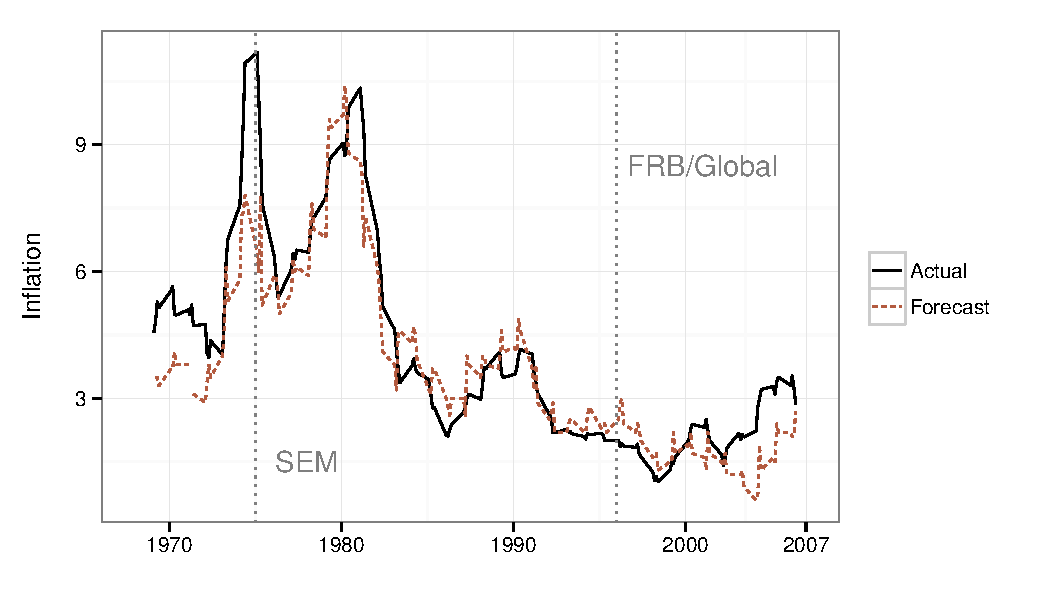
\includegraphics[width=0.8\linewidth]{figure/BaseInflation} 
\end{knitrout}

    
    \end{center}
    \begin{singlespace}
        {\scriptsize{Forecasts were made two quarters beforehand. \\
                     The grey dotted lines indicate the {\emph{approximate}} years that the Simultaneous Equation Models (SEM) and Federal Reserve Board Global (FRB/Global) forecasting models were fully implemented.  
                      }}
    \end{singlespace}
\end{figure}


\subsection{Are There Partisan Forecast Errors?}

































